\mysection{ТЕСТИРОВАНИЕ И АПРОБАЦИЯ РАЗРАБОТАННОЙ СИТЕМЫ}
\subsection{Функциональное тестирование}
Для тестирования было выбрано устройство Emlid Neutis N5.
Устройство представляет собой систему на модуле (System on Module, SoM), рассчитанную на разработчиков, проектирующих различные устройства для Интернета вещей и «умного» дома \cite{NEUTIS}.
Это устройство объединяет четыре ядра ARM Cortex-A53 и графический контроллер ARM Mali-450MP4 с поддержкой OpenGL ES 2.0/1.1, что позволит провести также тестирование полной версии образа \cite{NEUTIS}.

Функциональное тестирование приложения проводилось в ручном режиме.
\subsection{Конфигурация пакетов}
Для тестирования выходных образов системы сборки на выбранном устройстве необходимо сконфигурировать загрузчик и ядро Linux под выбранную платформу.
В данной главе в силу объемности конфигурационных файлов будет рассмотрена лишь процедура обновления пакета загрузчика для выбранной платформы.
Примеры конфигурирования и обновления прочих пакетов доступны в приложении к работе.
Обновление загрузчика осуществляется следующим образом:

1) Загрузка yocto слоя с патчами для загрузчика и ядра.

\lstinputlisting[
  caption={Загрузка yocto слоя}
]{source/meta-emlid-neutis.sh}

2) Загрузка и компиляция U-boot.

\lstinputlisting[
  caption={Загрузка U-boot},
  label={lst:pytest__short}
]{source/u-boot.sh}

\lstinputlisting[
  caption={Компиляция U-boot},
  label={lst:pytest__short}
]{source/u-boot-compile.sh}

2) Создание и установка .deb пакета с initramfs, установка пакетов загрузчика в образ.

\lstinputlisting[
  caption={Создание и установка пакета с initramfs},
  label={lst:pytest__short}
]{source/mkinitramfs.sh}

\lstinputlisting[
  caption={Установка загрузчика},
  label={lst:pytest__short}
]{source/u-boot-burn.sh}


\subsection{Запуск и апробация образа системы}
С помощью разработанной системы сборки были созданы три образа.
Были проверены следующие свойства полученных дистрибутивов:
\begin{itemize}
  \item Загрузка и работоспособность минимального образа;
  \item Загрузка и работоспособность серверного образа;
  \item Загрузка и работоспособность полного образа;
\end{itemize}
\begin{figure}[h!]
  \centering
  \setlength{\fboxsep}{5pt}
  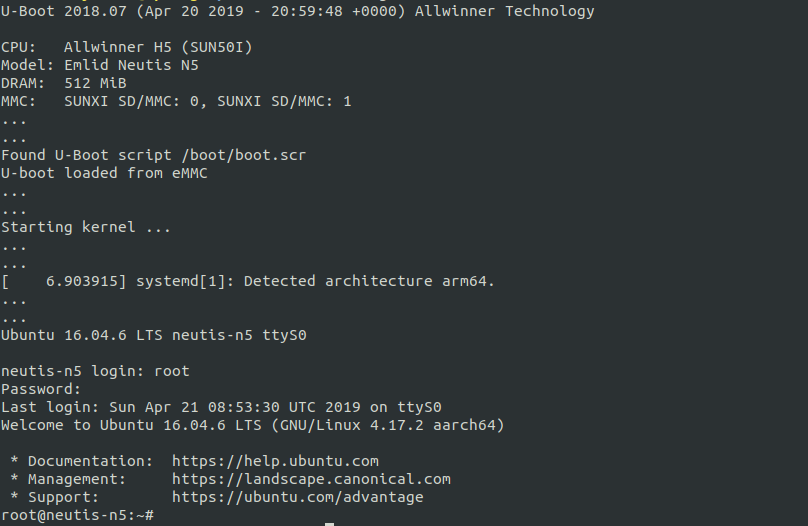
\includegraphics[height=10cm, width=15cm]{build/images/bootlog}
  \caption{Лог загрузки образа системы}\label{fig: bootlog}
\end{figure}

Кроме того, была проверена работоспособность системы сборки на Windows 10 Pro.

\newpage
